\documentclass[conference]{IEEEtran}

\usepackage{array}
\usepackage[brazil]{babel}
\usepackage[T1]{fontenc}
\usepackage[utf8]{inputenc}
\usepackage[pdftex]{graphicx}
\usepackage{hyperref}
\hyphenation{op-tical net-works semi-conduc-tor}


\begin{document}

\title{Panorama prático sobre estado atual dos bancos de dados ativos}

\author{\IEEEauthorblockN{Caio de freitas Valente\IEEEauthorrefmark{1}, Gabriel Reganati\IEEEauthorrefmark{2},  Rafael Reggiani Manzo\IEEEauthorrefmark{3}, Thiago de Gouveia Nunes\IEEEauthorrefmark{4}}
\IEEEauthorblockA{Instituto de Matemática e Estatística\\
Universidade de São Paulo\\
São Paulo, São Paulo\\
Emails:  \IEEEauthorrefmark{1}caiov@ime.usp.br, \IEEEauthorrefmark{2}reganati@ime.usp.br, \IEEEauthorrefmark{3}manzo@ime.usp.br, \IEEEauthorrefmark{4}nunes@ime.usp.br}
}

\maketitle
\IEEEpeerreviewmaketitle

\section{Introdução}
  \subsection{Motivação e contextualização}
  Em um sistema que utiliza um banco de dados relacional sem alguma ferramente ativa o controle de modificações sobre o banco de dados deve ficar na aplicação. Com a introdução dos banco de dados
  ativos é possível detectar modificações no banco de dados ou criar regras de monitoramento com base no tempo para controlar as transações que modificam o banco de dados. As grande vantagens
  de utilizar um sistema ativo dentro do banco de dados é:
  \begin{itemize}
    \item O ganho de eficácia, já que antes essas operações teriam que ficar na aplicação e agora são executadas dentro do SGBD. \\
    \item Agora o administrador de banco de dados pode ficar responsável em criar e manter essas regras, programando na mesma linguagem usada dentro do SGBD.\\
    \item Ao criar uma regra, ela fica dentro do banco de dados, onde outros usuários e aplicações podem acessá-la.
  \end{itemize}
  Atualmente vários banco de dados utilizados em larga escala comercialmente implementam de alguma forma o paradigma ativo. A \textit{Tabela III} mostra as principais ferramentas que implementam esse paradigma. A maioria dos SGBD modernos utilizam o conceito de \textit{Trigger} para criar uma regra ativa, que são detalhados na seção Estado da Arte.

  \subsection{Conceitos}
	Veremos adiante na seção \textit{Practical Applications of Triggers and Constraints: Successes and Lingering Issues} (\ref{subsubsec: article1}), uma breve descrição do porquê surgiram os bancos de dados ativos, alguns conceitos como o modelo ECA, Evento Condição Ação (\textit{Event Condition Action}), que serve como base para o uso de bancos de dados ativos, uma classificação de \textit{triggers} de acordo com a sua criação e atuação, veremos também uma forma de classificação que se baseia na funcionalidade do \textit{trigger}.

\section{Estado da arte}
  \subsection{Trabalhos científicos}
    \subsubsection{Practical Applications of Triggers and Constraints: Successes and Lingering Issues}\label{subsubsec: article1}
    
    \textit{Triggers} são baseadas no modelo ECA, quando um evento ocorre e alguma condição associada é verdadeira, executamos uma ação. Em relação ao seu comportamento, podemos definir muitas coisas como:
  
    \begin{itemize}
      \item \textbf{granularidade}: o \textit{trigger} age em nível de linha ou tabela;
      \item \textbf{ordem da ação}: se a ação deve ser executada antes, depois ou ao invés do evento que o disparou.
    \end{itemize}
  
    As condições e funções são definidas arbitrariamente. Note que podemos utilizar os valores que existiam antes do evento ser disparado e depois.

    \textit{Triggers} surgiram como uma forma de reação automática a violações de restrições de integridade, e logo foram generalizados para realização de outras tarefas, se tornando o modelo ECA que temos hoje. Os primeiros produtos que suportavam triggers surgiram no começo da década de 90, hoje em dia todos os fornecedores de SGBDs relacionais tem suporte a \textit{triggers}.

    Podemos ver uma classificação de \textit{triggers} na \textit{Tabela I}.

 \begin{table*}[!t]
    \renewcommand{\arraystretch}{1}
    \caption{Classificação por criação e atuação}
    \label{table_example}
    \centering
    \begin{tabular}{ c  c  c  c  }
      \hline 
	 & \bfseries DBMS Kernel & \bfseries DBMS Services & \bfseries External Applications \\
        \hline
            \bfseries Handcrafted &
            Gerenciamento de metadados, auditoria interna &
            NA &
            Regras de negócio, Escalonamento, Gerenciamento de fornecimento\\
	\hline
            \bfseries Generated &
            Integridade referencial, materialized views &
            Replicação, Extenders, Auditoria, Migração, Alertas &
            Gerenciamento de Workflow \\
	\hline
        \end{tabular}
    \end{table*}

    \begin{itemize}
        \item{Handcrafted}: São triggers criados por algum programador;
        \item{Generated}: Triggers gerados automaticamente;
        \item{Kernel}: Triggers escritos no Kernel, para não esbarrar em problemas de segurança ou então melhorar a performance;
        \item{Services}: Serviços que tem como proposito prover ou melhorar alguma funcionalidade do SGBD;
        \item{External}: Estão fora do banco de dados, fazem acesso ou se comunicam por meio de alguma API;
    \end{itemize}

    Podemos ainda classificar os \textit{triggers} em relação a sua função, como pode ser visto na \textit{Tabela II}.

 \begin{table*}[!t]
    \renewcommand{\arraystretch}{1}
    \caption{Classificação por função}
    \label{table_example}
    \centering
    \begin{tabular}{ c  c  }
      \hline 
           \bfseries Triggers preservador &
           Rollback caso as restrições sejam invalidadas \\
      \hline 
            \bfseries Triggers restaurador &
           Altera o valor para se conformar as restrições \\
      \hline 
            \bfseries Triggers sinalizador &
           Sinaliza para a aplicação, que deverá cuidar do problema \\
      \hline 
            \bfseries Materializing Trigger &
           Mantêm a consistência da materialized view \\
      \hline 
           \bfseries Metadata Trigger &
           Mantêm a consistencia dos metadados \\
      \hline 
           \bfseries Replication Trigger &
           Mantêm a consistencia de dados replicados de uma tabela para outra \\
      \hline 
           \bfseries Extenders &
           Gerencia novos tipos de dados e os mantêm consistentes com o banco de dados. \\
      \hline 
          \bfseries  Alerter &
           Notifica o usuário via manesagens \\
      \hline 
           \bfseries  Ad-Hoc Trigger &
            São triggers especificos para cada aplicação -> Regras de negócio, workflow, web, etc. \\
        \end{tabular}
    \end{table*}

    A grande vantagem do uso de \textit{triggers} é a possibilidade de mover a lógica e regras de negócio da aplicação para o banco de dados.

    Algumas das reclamações estão relacionadas à expressividade dos \textit{triggers}. Há certos problemas de padronização, como comportamentos particulares de cada SGBD com grande impacto nos resultados finais. Além disso, não há falta de ferramentas que ajudem na análise de \textit{triggers}, esse é um dos motivos que levou o crescimento de triggers gerados automaticamente. Muitos \textit{triggers}, ou \textit{triggers} complexos deterioram muito a performance.

    \subsubsection{\textit{Toward an Active Database Platform for Guiding Urban Pedestrians}}
    Utilizando a extensão \textit{PotsGIS} do sistema gerenciador de banco de dados (SGBD) PostgreSQL, que adiciona a capacidade de um tipo de dado para posição geográfica, este estudo da Universidade de Ume\r{a} na Suécia de autoria de Michael Minock, Johan Mollevik and Mattias \r{A}sander, através do uso extensivo de \textit{stored procedures} foi capaz de fornercer instruções de direção a fim de guiar um pedestre em um trajeto.

    Este banco de dados foi modelado para centralizar todo o estado do sistema como descrição dos mapas, posições do usuário, rotas e registro dos avisos enviados ao usuário. São basicamente quatro relações: \textit{PathNetwork}; \textit{Landmarks}; \textit{Routes}; e \textit{Pedestrian}.

    O primeiro uso de banco de dados ativo citado, é quando uma nova medição de \textit{GPS} é adicionada à base de dados, é disparado um \textit{trigger} que por sua vez executa uma \textit{stored procedure} que atualiza o estado do pedestre. Este tipo de ação é executado com alta frequência (uma vez por segundo).

    Estas modificações no estado do pedestre então podem desencadear outras regras para decidir quando enviar avisos sonoros ao pedestre, corrigir a rota quando o usuário sai do planejado, informar a distância restante e até mesmo encorajá-lo em sua caminhada. Tudo programado com \textit{triggers} e \textit{stored procedures}.

    Por outro lado, muitos destes eventos podem acontecer simultâneamente e para evitar que diversos avisos sejam disparados ao mesmo tempo, foi criada uma regra na inclusão da relação de avisos.

    Esta implementação obteve boa performance com atraso de resposta médio de 60ms. Quanto à precisão da navegação, os autores foram sinceros em dizer que ainda não está tão preciso quanto soluções a soluções de navegação comerciais. Mas também apontou quais pontos precisam ser melhorados para chegar a este ponto.

  \subsection{Ferramentas}
  Tabela comparativa
  \begin{table*}[!t]
    \renewcommand{\arraystretch}{1}
    \caption{Tabela de Ferramentas}
    \label{table_example}
    \centering
    \begin{tabular}{ c  c  c  c  c  c }
      \hline
      \bfseries Nome & \bfseries Trigger & \bfseries Primeiro release & \bfseries Última versão estável & \bfseries Último release & \bfseries Licensa \\
      \hline
      Apache Derby & Sim & 2004 & 10.10.1.1 & 2013 & Apache License \\
      \hline
      DB2 & Sim & 1983 & 10.5 & 2013 & Proprietária \\
      \hline
      H2 & Sim & 2005 & 1.3.171 & 2013 & EPL e modificação da MPL \\
      \hline
      HSQLDB & Sim & 2001 & 2.2.9 & 2013 & BSD \\
      \hline
      Microsoft Access (NET) & Sim & 1992 & 2013 & 2012 & Proprietária \\
      \hline
      Microsoft Azure SQL & Sim & 2010 & & 2012 & Proprietária \\
      \hline
      Microsoft SQL Server & Sim & 1989 & 2012 &  2012 &  Proprietária \\
      \hline
      Microsoft SQL Server Compact (Embedded Database) & Não & 2000 & 2011 & 2011 & Proprietária \\
      \hline
      MonetDB & Sim & 2004 & 11.9.1 & 2012 & MonetDB Public License v1.1 \\
      \hline
      MongoDB & Não & 2009 & 2.4.6 & 2013 & GNU AGPL v3.0 \\
      \hline
      MySQL & Sim & 1995 & 5.6.31 & 2013 & GPL ou Proprietária\\
      \hline
      Oracle & Sim & 1979 & 12c Release 1 & 2013 & Proprietária\\
      \hline
      Oracle Rdb  & Sim & 1984 & 7.2.5.3.0 & 2013 & Proprietária\\
      \hline
      PostgreSQL & Sim & 1989 & 9.3.1 & 2013 & PostgreSQL Licence (a liberal Open Source license) \\
      \hline
      RDM Embedded & Não & 1984 & 11.0 & 2012 & Proprietária \\
      \hline
      RDM Server & Sim & 1993 & 8.4 & 2012 & Proprietária \\
      \hline
      SQLite & Sim & 1905 & 3.8.0.2 & 2013 & Dominio Público \\
      \hline
      Xeround Cloud Database & Sim & 2010 & 3.1 & 2011 & SaaS \\
      \hline
    \end{tabular}
  \end{table*}

\section{Estudo de caso}
  \subsection{Características técnicas}
    \subsubsection{MS SQL}
    O Microsoft SQL Server é um SGBD - Sistema Gerenciador de Banco de dados relacional desenvolvido pela Microsoft. Em 1988 , a Microsoft lançou a primeira versão do SQL Server. Ele foi projetado para a plataforma OS / 2 e foi desenvolvido conjuntamente pela Microsoft e Sybase. Durante o início da década de 1990 , a Microsoft começou a desenvolver uma nova versão do SQL Server para a plataforma NT. Enquanto ele estava em desenvolvimento , a Microsoft decidiu que o SQL Server deve ser intimamente ligado com o sistema operacional NT. E desde então a Microsoft vem desenvolvendo e melhorando o sistema ano após ano e unicamente para o sistema operacional Windows. O SQL Server não é Open Source e para poder utilizar-lo é necessário comprar uma licença da Microsoft. Suas linguagens de consulta primárias são Transact-SQL (T-SQL) e ANSI SQL.\cite{sql-server-site} \cite{sql-server-site2}\\
    
    O SQL Server tem como principais características:
    \begin{itemize}
      \item Funciona no sistema operacional Windows
      \item Tem como tamanho máximo de banco de dados como 524 TB  e tamanho máximo de tabela como 524 TB
      \item Suporte a multi-threads
      \item A interface Connector/ODBC fornece ao SQL Server suporte a programas clientes que usam conexão ODBC (Open-DataBase-Connectivity).
      \item Suporte nativo ao XML
      \item Suporte a internacionalização
      \item Suporte a Data Warehouse
      \item Triggers Recursivas. É possível definir uma profundidade máxima de recursão
      \item Suporte a cryptografia
    \end{itemize}

	  Há dois tipos de consideração em SQL Server, AFTER e INSTEAD OF. AFTER não é executado até que as mudanças que o dispararam tenham feitos suas modificações nos dados, já o INSTEAD OF é executado após a criação das tabelas inserted (NEW) e deleted (OLD) forem criadas, mas antes de outras ações.\cite{caracteristica-mssql} \cite{caracteristica-mssql2}

    \subsubsection{MySQL}
	  MySQL é o mais popular sistema de gerenciamento de banco de dados SQL Open Source, é desenvolvido, distribuído e tem suporte da MySQL AB. A MySQL AB é uma empresa comercial, fundada pelos desenvolvedores do MySQL, cujos negócios é fornecer serviços relacionados ao sistema de gerenciamento de banco de dados MySQL\cite{mysql-site}\\

	  
    O MySQL tem como principais características:
    \begin{itemize}
      \item Escrito em C e C++.
      \item Funciona em diversas plataformas, como Windows, Linux 2.0+, OpenBSD, FreeBSD, SunOS 4.x e outros
      \item Utiliza o GNU Automake, Autoconf, e Libtool para portabilidade.
      \item Suporte total a multi-threads usando threads diretamente no kernel. Isto significa que se pode facilmente usar múltiplas CPUs, se disponível.
      \item Completo suporte a operadores e funções da linguagem SQL para consultas e funções
      \item Um sistema de privilégios e senhas que é muito flexível, seguro e que permite verificação baseada em estações/máquinas. Senhas são seguras porque todo o tráfico de senhas é criptografado quando você se conecta ao servidor.
      \item Os clientes podem se conectar ao servidor MySQL usando sockets TCP/IP, em qualquer plataforma.
      \item A interface Connector/ODBC fornece ao MySQL suporte a programas clientes que usam conexão ODBC (Open-DataBase-Connectivity). 
      \item O servidor pode apresentar mensagem de erros aos clientes em várias línguas. 
      \item Suporte total para vários conjuntos de caracteres, que incluem ISO-8859-1 (Latin1), big5, ujis e mais.
      \item Tem como tamanho máximo de banco de dados como ilimitado e tamanho máximo de tabela como 256 TB
    \end{itemize}
    A consideração e execução de regras ativas depende do tempo de execução definido para a trigger. Caso seja utilizada a clásula \textit{BEFORE} na \textit{trigger}, a consideração é feita antes da transação, enquanto que no caso de \textit{AFTER} ela é feita após a transação. Já a execução é sempre imediata.\cite{caracteristica-myssql}

  \subsection{Cenário}
    \subsubsection{O Problema}
    Ao se deparar com a criação de um sistema web o qual realizaria a venda de papel moeda e cartões pré-pagos internacionais pela internet, teve-se que pensar em como fazer a atualização das taxas de moedas a serem vendidas a partir de um serviço externo com atualizações periódicas, que consistem de chamadas bastante demoradas tanto pelo volume de dados quanto pelo tempo de resposta do serviço externo.\\
    Além disso a compra de cambio apresenta uma validade de 2 dias, portanto o banco de dados deveria ser possível cancelar a compra caso não fosse efetuada no período de dois dias.

    \subsubsection{A Solução}
    Para que a cada requisição de um usuário pela taxa de câmbio de uma moeda não resulte em uma requisição deste tipo para um serviço externo, foi pensada uma tabela de \textit{cache} para as cotações que por é atualizada por meio de regras ativas. Assim, ao invés de acessar um serviço externo, a operação de obter a taxa de câmbio consiste de uma simples consulta a tabela.\\
    Com o intuito de solucionar o problema da validade foram feitas \textit{triggers} que façam esse tipo de análise e assim trocando validando ou não a compra.

  \subsection{Descição dos testes}
  A fim de aferir as capacidades dos SGBDs SQLServer e MySQL quanto a utilização de regras ativas, e tendo em mente o cenário anteriormente descrito, foram elaborados dois casos de teste a serem realizados em ambas os sistemas:

  \begin{enumerate}
    \item Execução periódica de uma regra para atualizar as informações sobre taxa de câmbio;
    \item Invalidãção de compras realizadas há mais de dois dias.
  \end{enumerate}

  \subsection{Modelagens}

    Toda modelagem que fizemos pode ser encontrada no seguinte link: \href{https://github.com/gorobaum/t2bd/}{https://github.com/gorobaum/t2bd/}.

    \subsubsection{MySQL}
    Para os testes com o SGBD MySQL, foi adotada a seguinte modelagem com quatro relações: Boleto; Cambio; Taxa; e Moeda.

    A relação Boleto representa uma operação de compra realizada, contendo os atributos id, data, pago (booleano), valor e id\_cambio.

    Por sua vez a relação Cambio representa as taxas do dia de uma dada moeda para outra com atributos id, id\_taxa\_origem, id\_taxa\_destino.

    Assim como deve ter sido possível inferir pelo nome, a relação Taxa, com atributos id, data, id\_moeda e valor, representa uma taxa de conversão para uma dada moeda em uma dada data.

    Por fim, a relação Moeda contém apenas o nome desta e sua id.

    Neste foi criado uma regra ativa para que, quando uma taxa é inserida, todos os boletos vencidos sejam removidos.

    \begin{figure}[!t]
      \centering
      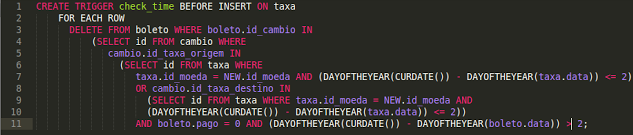
\includegraphics[scale=0.40]{img/trigger-mysql.png}
      \caption{Modelagem do banco MS SQL para os testes}
    \end{figure}

    \subsubsection{SQLServer}
  	Usamos a ferramenta SQL Server Management Studio para trabalhar com SQL Server.			
  	Decidimos seguir o mesmo padrão usado na resolução do problema com MySQL, segue o diagrama das tabelas:
   
    \begin{figure}[!t]
      \centering
      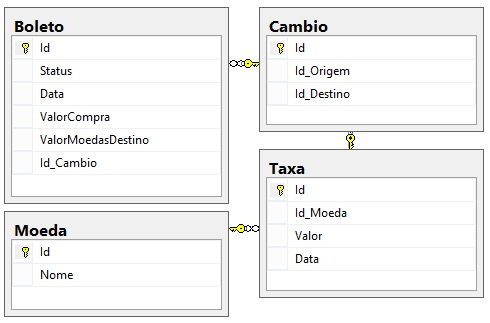
\includegraphics[scale=0.65]{img/tabela.jpg}
      \caption{Modelagem do banco MS SQL para os testes}
    \end{figure}

  	Em seguida desenvolvemos uma aplicação web que a partir do nome de uma moeda busca a taxa de cambio em relação ao Real. Esse valor já parseado é retornado\footnote{\href{http://trabalho2db.azurewebsites.net/Currency/Get?exchangeRate=}{http://trabalho2db.azurewebsites.net/Currency/Get?exchangeRate=}}.

    \begin{figure}[!t]
      \centering
  	  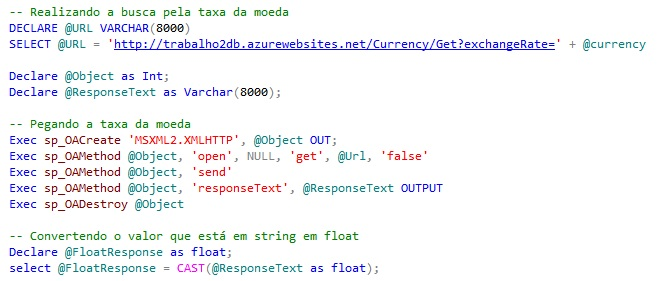
\includegraphics[scale=0.65]{img/requisicao.jpg}
      \caption{Código para em T-SQL para requisição web}
    \end{figure}

  	Criamos o stored procedure AtualizaTaxa, que para toda entrada na tabela Moeda envia o valor seu nome para a aplicação web, e cria uma nova entrada em taxa com seu horário da atualização e valor obtido.

  	O próximo passo foi criar o stored procedure AtualizaTaxaDeCambio para associar as taxas de todas as moedas que foram obtidas mais recentemente em todas as possíveis combinações de origens e destinos, por exemplo supondo que temos no banco de dados a taxa das seguintes moedas: USD, EUR e BRL vamos obter em Cambio as seguintes combinações: USD-USD, USD-EUR, USD-BRL, EUR-USD, EUR-EUR, EUR-BRL, BRL-USD, BRL-EUR, BRL-BRL.

  	Os dois stored procedures acima são executados de cinco em cinco minutos. SQL Server não suporta \textit{triggers} temporais diretamente, mas podemos fazer uma construção equivalente usando Jobs. 

    \begin{figure}[!t]
      \centering
  	  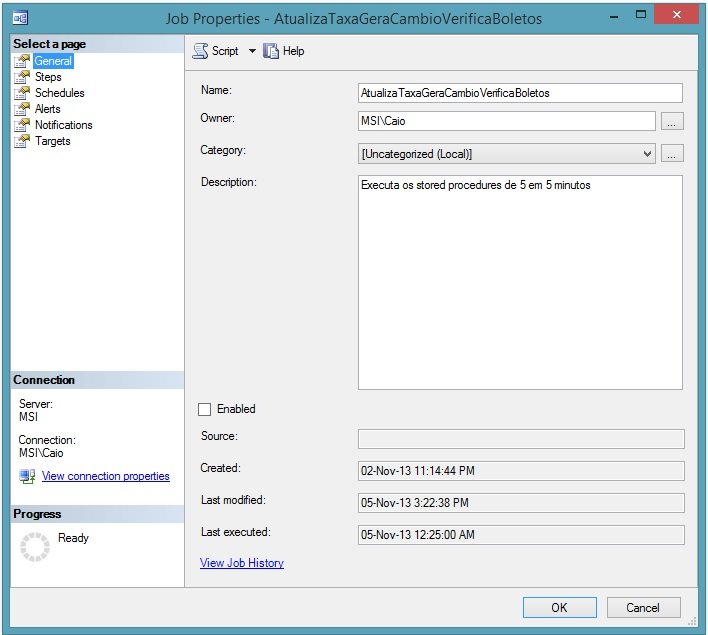
\includegraphics[scale=0.45]{img/job1.jpg}
      \caption{Primeiro passo da criação de uma job MS SQL}
    \end{figure}

  	Jobs são conjuntos de operações. Um job pode executar diversas atividades, incluindo scripts T-SQL ou queries. Ao final de cada atividade sabemos se a atividade foi bem sucedida ou mal sucedida, a partir disso podemos definir um fluxo de execução para o job.
  	
    \begin{figure}[!t]
      \centering
  	  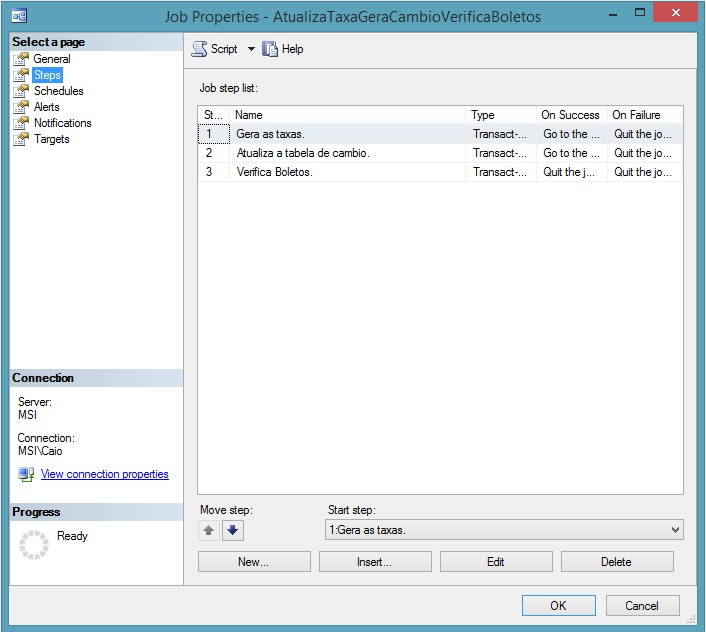
\includegraphics[scale=0.45]{img/job2.jpg}
      \caption{Segundo passo da criação de uma job MS SQL}
    \end{figure}

  	Jobs podem ser escalonados para executarem em algum horário ou alguma frequência desejada.

    \begin{figure}[!t]
      \centering
  	  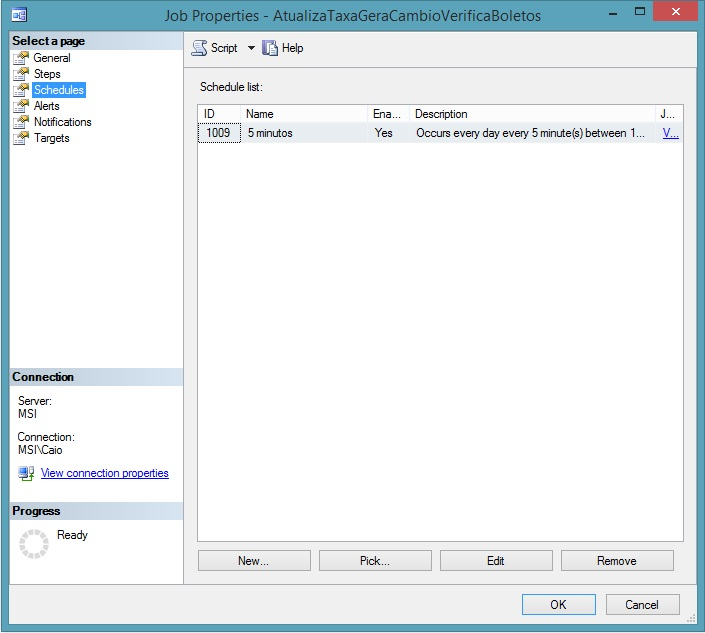
\includegraphics[scale=0.45]{img/job3.jpg}
      \caption{Terceiro passo da criação de uma job MS SQL}
    \end{figure}

  	Note que além de podermos criar um job usando a IDE, podemos também fazer por meio de código.

  	Quando o usuário realiza uma compra, é especificado o valor em moedas destino que deseja comprar, usando essa informação e as informações de cambio mais recentes podemos calcular o valor da compra usando um trigger:

    \begin{figure}[!t]
      \centering
  	  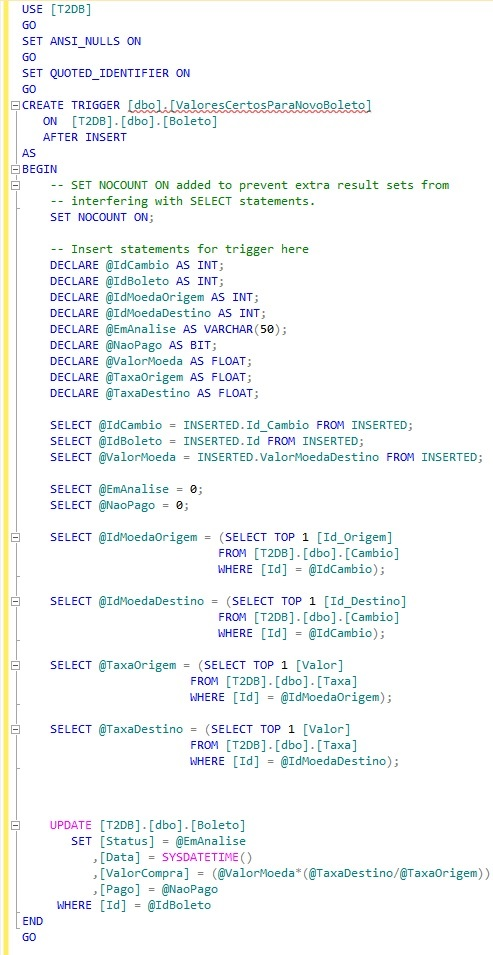
\includegraphics[scale=0.6]{img/trigger.jpg}
      \caption{Descrição do trigger em MS SQL para atualizar os valores de boleto}
    \end{figure} 

    O status da compra fica pendente até o usuário pagar o valor da compra, e nesse caso o status passa para finalizado, ou então até dois dias após o início da transação e nesse caso usamos um job para alterar o status do boleto para cancelado.

  \subsection{Conclusão dos testes}
  Conseguimos concluir a tarefa nos dois SGBDs com ressalva de que com o MySQL não foi possível fazer uma requisição externa diretamente.

	Cada sistema apresenta particularidades, principalmente a sintaxe. Com o MS SQL precisamos usar stored procedures e Jobs além de \textit{triggers}, já em MySQL foi possível realizar a tarefa usando apenas \textit{triggers}.

	Constatamos também que com o uso de SGBDs ativos foi possível transferir a lógica da aplicação para o banco de dados.

\section{Conclusão}
Esperamos com este artigo ter demonstrado o poder que regras ativas possuem, sendo capaz desde produzir um sistema de navegação até atualizar cotações de moeda rapidamente.

Da mesma forma, foi no artigo foi aprofundada a teoria sobre regras ativas com detalhes do modelo ECA, classificação do tipo quanto a sua origem e mais.

Por fim, o estudo de caso demonstrou como se implementar em dois sistemas gerenciadores bastante diferentes que foram o MS SQL e MySQL.

\begin{thebibliography}{1}

  \bibitem{Practical Applications of Triggers and Constraints: Successes and Lingering Issues}
  S. Ceri, R. J. Cochrane, J Widom, \textit{Practical Applications of Triggers and Constraints: Successes and Lingering Issues}, VLDB conference, Cairo Egypt. 2000.

  \bibitem{sweedish-article}
  M. Minock, J. Mollevik and M. \r{A}sander, \textit{Toward an Active Database Platform for Guiding Urban Pedestrians}. Ume\r{a}, Sweden: University of Ume\r{a}, 2012.

  \bibitem{sql-server-site}
http://msdn.microsoft.com/en-us/library/hh231622.aspx
  
\bibitem{sql-server-site2}
http://www.informit.com/articles/article.aspx?p=30167

  \bibitem{mysql-site}
  http://ftp.nchu.edu.tw/MySQL/doc/refman/4.1/pt/

  \bibitem{caracteristica-myssql}
  http://www.cs.duke.edu/csl/docs/mysql-refman/triggers.html

  \bibitem{caracteristica-mssql}
http://searchsqlserver.techtarget.com/feature/Designing-and-implementing-triggers-in-Microsoft-SQL-Server

  \bibitem{caracteristica-mssql2}
http://msdn.microsoft.com/en-gb/magazine/cc164047.aspx


\end{thebibliography}

\end{document}
